\documentclass[times, utf8, zavrsni]{fer}
\usepackage{booktabs}
\usepackage{pdfpages}

\begin{document}

% TODO: Navedite broj rada.
\thesisnumber{482}

% TODO: Navedite naslov rada.
\title{Korespondencijska ugrađivanja za stereoskopsku rekonstrukciju}

% TODO: Navedite vaše ime i prezime.
\author{David Kerman}

\maketitle

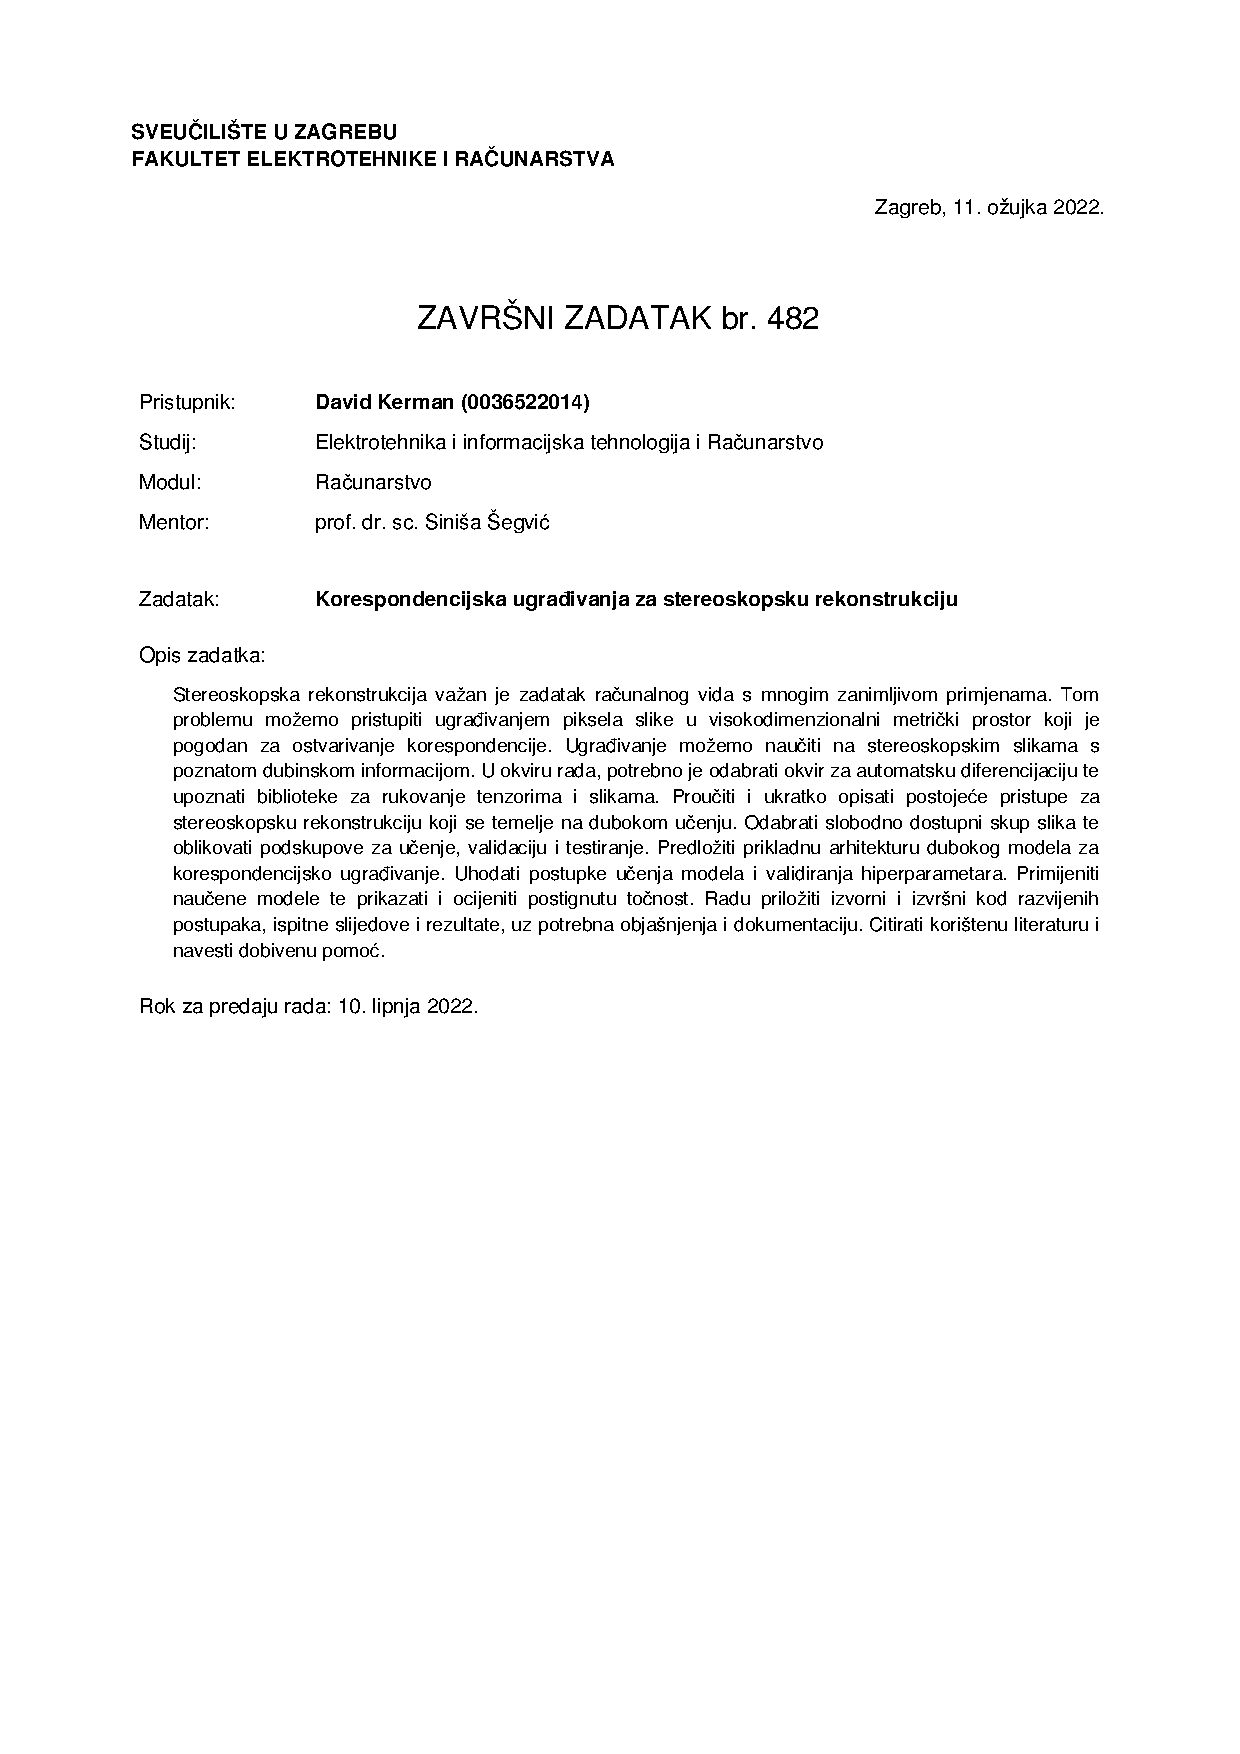
\includepdf[pages=-]{izvornik.pdf}

% Dodavanje zahvale ili prazne stranice. Ako ne želite dodati zahvalu, naredbu ostavite radi prazne stranice.
\zahvala{Zahvaljujem mentoru prof.~dr.~sc.~Siniši Šegviću, na savjetima i ukazanoj pomoći. Također, zahvaljujem svojoj obitelji, prijateljima i kolegama na potpori tijekom mojeg dosadašnjeg obrazovanja.}

\tableofcontents

\chapter{Uvod}
Računalni vid kao jedna od temeljnih grana umjetne inteligencije omogućava računalima da izluče značajnu informaciju iz slika, videa ili sličnih vizualnih ulaza. Područje stereoskopske rekonstrukcije ima za cilj ostvariti stvaran trodimenzionalan položaj točaka koje su promatrane u dvije ili više slika, te kao takvo ima vrlo široke primjene uključujući one za određivanje sličnosti slikovnih okana. Kroz povijest postojale su klasične metode za određivanje korespodencijskih metrika, no pojavom snažnijih računala iskorišteno je duboko učenje kao alat kojim je moguće korespodencijske metrike naučiti na stvarnim podacima. Za potrebe metoda temeljenih na ugrađivanju u visokodimenzionalni prostor potrebne su rektificirane stereoskopske slike s poznatom dubinskom informacijom.\\

U okviru ovog radu opisana je geometrija stereoskopskog para, kalibracija, rektifikacija i algoritmi korišteni za ostvarivanje korespodencije. Zatim definirani su osnovni pojmovi u dubokom učenju, te postupci korišteni u dubokom učenju uz memorijske zahtjeve. Predstavljen je podatkovni skup na kojem su izvršeni postupci treniranja i validacije. Opisan je model kojim je ostvareno korespodencijsko ugrađivanje slikovnih okana, koji su korišteni u stereoskopskoj rekonstrukciji. Nastavno na to, opisan je postupak učenja takvog modela, te eksperimentalno vrednovanje rekonstrukcijske točnosti.

\chapter{Stereoskopska rekonstrukcija}
\section{Epipolarna geometrija}
Epipolarna geometrija je geometrija koja ima primjenu u stereoskopskoj rekonstrukciji, a po definiciji opisuje odnos točaka u slikama dobivenih iz dviju kamera. Također naziva se i epipolarno ograničenje jer uvelike smanjuje broj točaka koje je potrebno provjeriti pri traženju korespodentnih točaka. Točka $X$ koja je prikazana na slici 2.1 prikazuje točku u 3D prostoru koja se snima iz dviju kamera. Točke $C$ i $C'$ prikazuju centre lijeve, odnosno desne kamere. Projekcija točke $X$ na ravninu lijeve kamere je $x$, a na ravninu desne kamere $x'$. Važno je napomenuti da su točke $X$, $x$ i $x'$ u istoj ravnini, te zajedno sa centrima kamera $C$ i $C'$ čine tzv. \textit{epipolarnu ravninu} $\pi$.\\
\begin{figure}[htb]
\centering
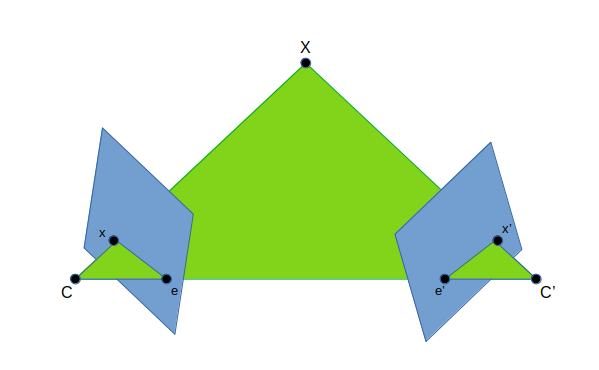
\includegraphics[scale=0.46]{img/slika1.png}
\caption{Epipolarna ravnina u kojoj se nalaze točka $X$,te točke nastale projekcijom $x$ i $x'$}
\label{fig:Epipolar}
\end{figure}\\
Nadalje, na slici su označeni \textit{epipolovi} oznakama $e$ i $e'$ te oni prikazuju točke u kojima pravac koji povezuje centre kamera $C$ i $C'$ siječe slikovne ravnine.
Najvažniji element su \textit{epipolarne linije}, označene dužinama koje spajaju $x$ i $e$, te $x'$ i $e'$, ali su zapravo pravci koji su nastali presjekom epipolarne ravnine sa slikovnom ravninom. Epipol je točka u kojoj se sijeku svi epipolarni pravci.\\
Poznavajući činjenicu da se točke nalaze u istoj ravnini, te ako znamo položaj točke $x$ možemo odrediti položaj točke $x'$. Rješenja koja se moraju ispitati da bi saznali položaj točke $x'$ nalaze se na epipolarnoj liniji, što uvelike olakšava pronalaženje korespodentnih točaka.

\section{Pretprocesiranje slika}
Parametre geometrije sustava kamera moguće je  podijeliti na dvije vrste: intrinzični i ekstrinzični. Ekstrinzični parametri su oni koji opisuju odnos svojstva koja su zajednička kamerama. Intrinzični pak opisuju svojstva kamera koje se odnose svaku kameru pojedinačno. Kao primjere za intrinzične faktore navodimo svojstva koja utječu na nji, a to su nesavršenost leća (na slici 2.2 prikazano je radijalno izobličenje), pomak senzora od centra leća te slične fizičke karakteristike nesavršenosti kamera.\\
\begin{figure}[htb]
\centering
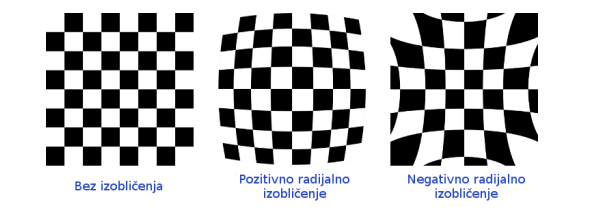
\includegraphics[scale=0.7]{img/slika2.png}
\caption{Primjeri radijalnog izobličenja. Izvor:[1]}
\label{fig:Radial}
\end{figure}\\
S druge strane ekstrinzični parametri nas dovode do nužnih transformacija kojima se slike dovode u istu ravninu projekcije te se time postiže da su pikseli duž horizontalnog pravca jedne slike na istoj visini na drugoj slici. Taj pravac je već spomenut, riječ je o epipolarnoj liniji. Ovakvim transformacijama uvelike se olakšava pronalaženje korespodentnih točaka koje u ovom slučaju treba tražiti samo duž jedne linije, epipolarne linije. Problem je sveden na jednu dimenziju. Kalibracijom se riješava problem nesavršenosti leća, odnosno problem izobličenja slika.\\
\\

\subsection{Rektifikacija}
Za postupak rektifikacije važni su ekstrinzični faktori kamera, dok na njihov izračun utječu intrinzični faktori. Transformacijom slika rektifikacijom dobivamo slike čiji pikseli koji u prostoru odgovaraju točkama na istoj visini,a nalaze se duž iste epipolarne linije. Također, nakon provedenih transformacija intrinzični parametri kamera postaju jednaki.\\
\begin{figure}[htb]
\centering
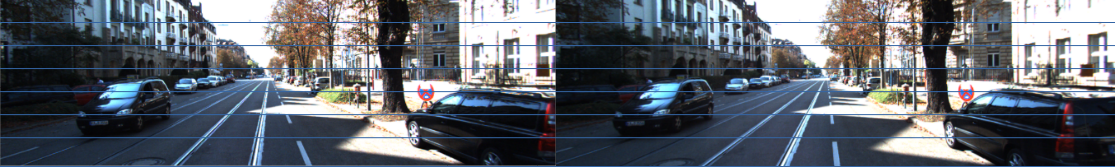
\includegraphics[width = 14.5cm]{img/slika3.png}
\caption{Prikaz epipolarnih linija u rektificiranim slikama skupa KITTI 2015}
\label{fig:Radial}
\end{figure}\\
Postupak se provodi kroz nekoliko koraka, a uključuje šahovsku ploču koja je pogodna zbog svojih svojstava. Prvi korak je traženje šahovskih polja. Postupak se nastavlja određivanjem izobličenja i ostalih parametara uz pomoć šahovskih polja.
Na slici 2.2 prikazan je par slika iz stereo kamera koji je rektificiran. Slike su iz skupa KITTI 2015, te se na njima vide epipolarne linije. Lako je primjetiti da iste točke u prostou nalaze na istoj visini, odnosno na istoj epipolarnoj liniji. Ovakvom transformacijom, korespodentne piksele potrebno je tražiti samo na istoj $y$-koordinati.

\section{Disparitet}
Prijašnjim postupcima kalibracije i rektifikacije omogućen je postupak računanja dispariteta, odnosno postupak računanja koji za svaki piksel koji je nastao lijevom kamerom određuje piksel slike koja je nastala desnom kamerom, ali pomaknutog za udaljenost $d$ piksela po horizonatlnoj osi. \textit{Disparitet} je definiran kao horizontalni pomak $d$ između dvaju korespodentnih piksela u slikama nastalim iz dviju konkurentnih stereo kamera. Kao rezultat računanja dispariteta nastaje mapa dispariteta koja sadrži disparitet za svaki piksel referentne kamere. Odnos piksela slike iz lijeve kamere, koja je u ovom slučaju referentna, i slike iz desne kamere definira se kao: 
\begin{equation}
I_{L}(x, y) = I_{D}(x-d,y)
\label{eq:Disparitet}
\end{equation}
gdje su $I_{L}$ i $I_{D}$ slike nastale lijevom, odnosno desnom kamerom, respektivno. Uređenim parom $(x,y)$ opisani su pikseli slike iz lijeve kamere, a njemu korespodentni pikseli u slikama iz desne kamere označeni su pomakom za disparitet $d$ po horizontalnoj osi $(x-d,y)$. Važno je napomenuti da su slike u skupu KITTI 2015 rektificirane i kalibrirane, što znači da korespodentne piksele tražimo samo po horizontalnoj osi.
Pomoću izračunatog dispariteta moguće je izraziti odnos između piksela kamera i dubine scene kao:
\begin{equation}
Z=f\frac{B}{d}
\label{eq:Fokalna}
\end{equation}
gdje je dubina scene, odnosno udaljenost objekta od kamere označena sa $Z$, $d$ je disparitet,s $B$ je označnena udaljenost između središta kamera, a s $f$ je označena fokalna udaljenost kamere. Iz jednadžbe 2.2 je vidljiva obrnuta proporcionalnost između udaljenosti objekta od kamera, te dispariteta s druge strane. Kada je položaj objekta blizu kamere, disparitet će biti velik. A kako se udaljavamo od kamere, disparitet se smanjuje i u beskonačnosti postiže vrijednost 0.\\
Na slici 2.4. je vidljivo da su epipolarne linije paralelne, te im je $y$-koordinata za korespodentne piksele jednaka. Disparitet je označen slovom $d$ i prikazuje horizontalni pomak.
\begin{figure}[htb]
\centering
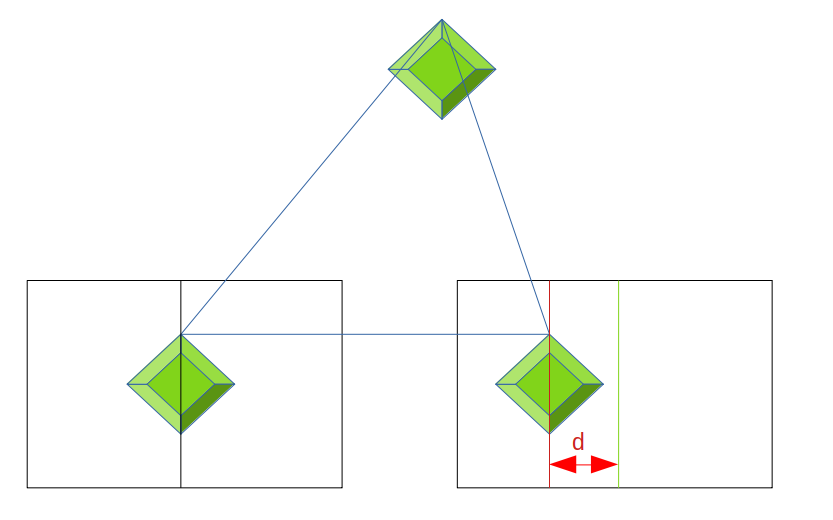
\includegraphics[width = 14.5cm]{img/slika4.png}
\caption{Prikaz objekta u slikama iz lijeve i desne kamere. Plavom bojom označena je epipolarna ravnina. Okomitim osima označeni su projicirani pikseli u konkuretnim slikama. Disparitet je označen slovom $d$.}
\label{fig:Disparitet i epipolar}
\end{figure}\\
\\\\
\section{Algoritam stereoskopske rekonstrukcije}
Postupak stereoskopske korespodencije je zapravo postupak pronalaženja istih piksela u međusobno konkurentnim kamerama koji odgovaraju istoj točki u trodimenzionalnom prostoru. Postoje dvije vrste korespodencija, \textit{rijetke} i \textit{guste}. Razlika je u tome što rijetke ne izračunavaju disparitete za sve piksele, dok guste to rade. Guste korespodencije omogućene su današnjom snagom računala, te se rijetke više toliko ne koriste. Postupak guste korespodencije je tim teži što se prilikom izračuna susreće s nekim anomalijama u slikama, primjerice područjima bez teksture, reflesivnim podlogama na kojima se svjetlost drugačije lomi i odbija, te točkama koje se iz jedne kamere vide, a iz druge ne (\textit{stereoskopska sjena}).\\
Dolazimo do stereo algoritama, svaki od njih moguće je opisati u četiri koraka ([2],[3]):
\begin{enumerate}
\item izračunavanje razlike između dvaju slikovnih okana, odnosno izračun podatkovnih cijena po prije definiranoj mjeri razlike
\item prikupljanje podatkovnih cijena za disparitete koji se razmatraju
\item izračun mape dispariteta, odnosno odabir najmanje prikupljene cijene za svaki piksel, uz optimizaciju
\item zaglađivanje mape dispariteta 
\end{enumerate}

Prvi korak ovog generičkog algoritma za stereoskopsku rekonstrukciju je izračun podatkovnih cijena. Izračun podatkovnih cijena može se računati prema pojedinačnim pikselima ili skupini piksela.  Izračun nam govori kolika je razlika između dvaju slikovnim okana, a razlika koja se koristi je definirana prije. Mjere razlike mogu biti sljedeće:
\begin{itemize}
\item[•] srednja kvadratna razlika
\item[•] srednja apsolutna razlika
\item[•] kvadratna razlika između intenziteta piksela
\item[•] apsolutna razlika između intenziteta piksela
\end{itemize}

\newpage
Drugi od koraka generičkog stereo algoritma je prikupljanje podatkovni cijena, tj. agregacija.  Na početku je postavljena granica za maksimalan disparitet, pa se tijekom ovogg koraka izračunava podatkovna cijena za sve disparitete i skupa  od $0$ do $D$, te ćemo tako za svaki piksel imati $D+1$ podatkovnih cijena.\\
Treći korak algoritma je izračun mape dispariteta. Nakon što su izračunate podatkovne cijene za razmatran skup dispariteta, treba odabrati metodu za izračun mape dispariteta. U praksi postoje \textit{lokalne} i \textit{globalne}. Lokalne metode prikupljaju cijene nad ograničenim područjem unutar same mape dispariteta, odnosno traže na ograničenom području oko referentne točke. Područje moje biti 2D ili 3D, te se prikupljanje može primjerice izvesti konvolucijom. S druge strane, globalne metode  preskaču korak prikupljanja podatkovnih cijena, te odmah nakon izračuna podatkovnih cijena vrše optimizaciju. Globalne metode minimiziraju kriterij nad cijelom slikom. Odnos između ovi metoda može se svesti na to da su lokalne brže, no globalne daju puno glađe mape dispariteta, što ih čini kvalitetnijima.\\
Zadnji korak koji je naveden je zaglađivanje mapa dispariteta. Ovaj korak je opcionalan i neke metode ga koriste. Glavni cilj ovog koraka je uklanjanje šuma koji je nastao generiranjem mape. 
\chapter{Duboko učenje}
\section{Osnovni pojmovi u dubokom učenju}
\subsection{Perceptron}
\subsection{Prijenosne funkcije}
\subsection{Konvolucijski slojevi}
\subsection{Optimizacija}
\subsection{Regularizacija}
\section{Učenje dubokih modela}
\subsection{Funkcija gubitka}
\subsection{Gradijentni spust}
\subsection{Memorijska zahtjevnost}
\chapter{Podatkovni skup za učenje}
\section{Podatkovni skup KITTI 2015}
\chapter{Duboko učenje u kontekstu stereoskopske rekonstrukcije}
\section{Ugrađivanje okana u metrički prostor}
\section{Učenje modela za ostvarivanje korespodencije}
\chapter{Eksperimentalni rezultati}
\chapter{Programska izvedba i vanjske biblioteke}

\chapter{Zaključak}
Zaključak.

\bibliography{literatura}
\bibliographystyle{fer}

\begin{sazetak}
Sažetak na hrvatskom jeziku.

\kljucnerijeci{Ključne riječi, odvojene zarezima.}
\end{sazetak}

% TODO: Navedite naslov na engleskom jeziku.
\engtitle{Title}
\begin{abstract}
Abstract.

\keywords{Keywords.}
\end{abstract}

\end{document}
